\chapter{Courant électrique}

\section{Courant électrique}

\marginnote{
  Tremblay \S 5.1, 5.2

  Lafrance \S 6.1
}

\paragraph{Objectif}

\begin{enumerate}
  \item L'étudiant analysera un modèle de conduction impliquant la vitesse de
    dérive des électrons dans un conducteur.
\end{enumerate}


Le courant donne la quantité de charge par unité de temps qui traverse un fil
$$i_\mathrm{moy} \equiv \abs{\frac{\Delta Q}{\Delta t}}$$
En général, cette quantité peut fluctuer et la définition générale est
$$i \equiv \abs{\frac{dQ}{dt}}$$

La direction du courant est la direction des charges positives.


\subsection{Vitesse de dérive}

Regardons de plus près des électrons de conduction dans un fil.

Ils se déplacent dans des directions aléatoires. En première approximation, on
peut considérer les électrons de conduction comme formant un gaz parfait.
D'après le théorème d'équipartition en thermodynamique, l'énergie des électrons
est
$$\frac{3}{2} kT$$
ce qui permet de déterminer que leur vitesse thermique est de l'ordre de
\SI{1e5}{m\per s}.

Avec une différence de potentiel, les électrons se déplaceront légèrement plus
vers le potentiel le plus élevé. La vitesse thermique demeure et les collisions
aussi. Dans l'ensemble, la vitesse effective avec laquelle les électrons se
déplacent vers le potentiel positif est appelée la \textbf{vitesse de dérive}.
En général, la vitesse de dérive est de l'ordre de \SI{1e-6}{m\per s}.


\subsection{Courant et vitesse de dérive}

Considérons une section de fil de surface $A$. Dans un intervalle de temps
$dt$, seul les électrons qui se trouvent à une distance inférieure à $v_d
dt$ pourront traverser la section de fil. Combien d'électron de
conduction y a-t-il?
Supposons qu'il y en a $n$ par unité de volume dans le fil. La charge totale
qui peut traverser la surface est donc
\begin{align*}
  dQ = -env_ddt A
\end{align*}
d'où
\begin{align*}
  i = env_d A
\end{align*}

\begin{center}
  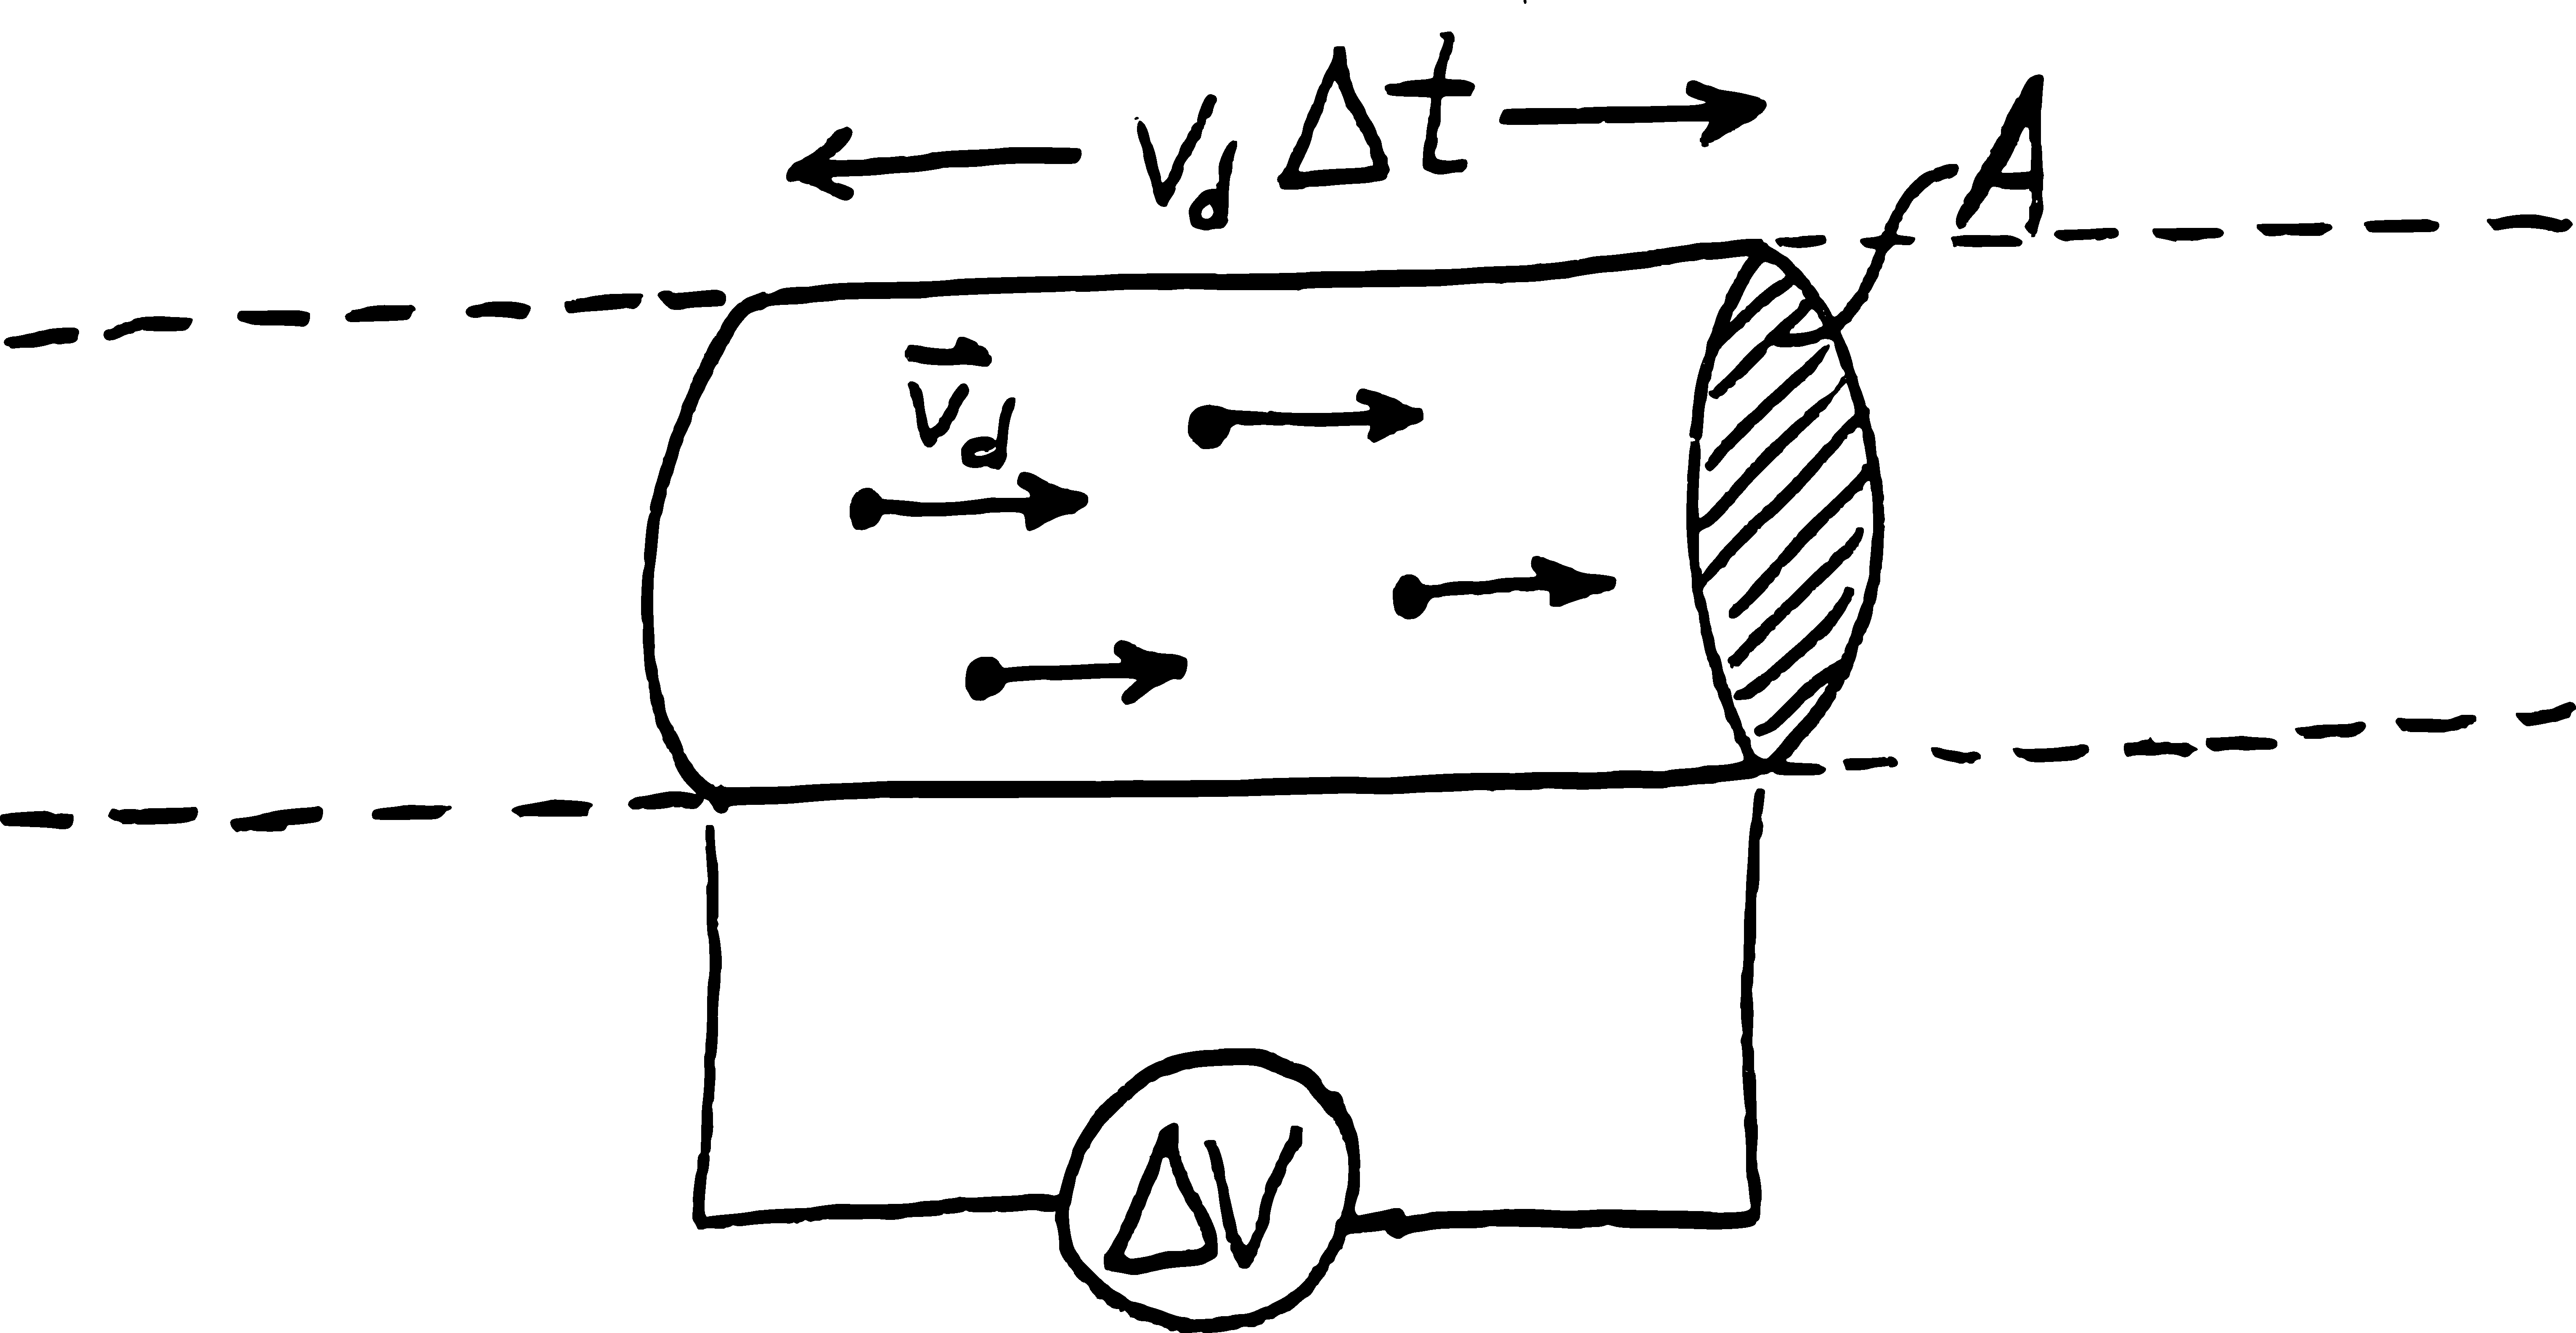
\includegraphics[width=5cm]{06-courant/figures/courant-vd.pdf}
\end{center}

On définit la \textbf{densité de courant} par
\begin{align*}
  J &\equiv \frac{i}{A} \\
    &= env_d
\end{align*}



\section{Modèle de conduction et résistance}

\marginnote{
  Tremblay \S 5.3

  Lafrance \S 6.2, 6.4, 6.5
}
Qu'en est-il de la vitesse de dérive? On se doute qu'elle dépend du champ
électrique, mais comment? D'abord, clarifions le fait qu'il existe un champ
électrique dans le fil même si c'est un conducteur. En effet, il y a des
charges qui bougent, donc la situation n'est pas à l'équilibre électrostatique.
Si le champ électrique est constant, on s'attend à ce que la force électrique
sur les charges en mouvement soit constante et donc que l'accélération des
charges soit constante. Si c'était le cas, on aurait une vitesse de dérive qui
augmente continuellement. Ce n'est pas ce qui est observé. On constate plutôt
que la vitesse de dérive est constante. Ceci est causé par les nombreuses
collisions que les charges en mouvement subissent lors de leur déplacement. Ces
collisions sont équivalentes à un mouvement dans un milieu résistant, comme une
voiture qui se déplace dans l'air. Si le milieu exerce une force
proportionnelle à la vitesse, on peut montrer que les charges atteindront une
vitesse limite constante. On a donc que
\[
  v_d = \mu_e E
\]
où $\mu_e$ est une constante de proportionnalité, la \textbf{mobilité} des
électrons. En combinant avec le résultat obtenu plus haut, on obtient la
relation suivante entre le courant et le champ électrique
\[
  i = en\mu_e AE.
\]
En terme de la densité de courant, on obtient
\[
  J = en\mu_e E.
\]
On définit la constante
\[
  \rho \equiv \frac{1}{en\mu_e}
\]
comme étant la \textbf{résistivité} du matériau.


Si on applique une différence de potentiel $\Delta V$ entre deux extrémités
d'un fil de longueur $l$ et de section $A$, le champ électrique est
$$E = \frac{\Delta V}{l}$$
donc la densité de courant est
$$J = \frac{1}{\rho l} \Delta V$$
et le courant est
$$I = JA = \frac{A}{\rho l} \Delta V.$$

On définit la \textbf{résistance} d'un matériau comme le rapport de la
différence de potentiel sur le courant:
\[
  R = \frac{\Delta V}{I}.
\]

À partir de la relation ci-haut, on a donc
\[
  R = \frac{\rho l}{A}
\]

Un matériel pour lequel la résistance est indépendante de la différence de
potentiel est appelé un matériel ohmique. On dit que ce matériel satisfait la
\textbf{loi d'Ohm}, c'est-à-dire que la relation entre la tension et le courant
est linéaire.



\section{Puissance}

\marginpar{Tremblay \S 5.4}

La puissance est l'énergie dissipée (ou fournie) par unité de temps. On sait
que si une charge $dq$ se déplace entre deux points séparés par une différence de
potentiel $\Delta V$, l'énergie potentielle changera de
$$dU = \Delta V dq.$$
L'énergie cinétique demeurera constante si on suppose que le courant est
uniforme entre les deux points qui nous intéressent (ce qui est souvent le
cas). Par conséquent, le taux de variation de l'énergie dans le temps est
\begin{align*}
  P &= \frac{dU}{dt} \\
    &= \frac{\Delta V dq}{dt} \\
    &= \Delta V I \\
    &= RI^2
\end{align*}


\subsection*{Exercice}

\marginpar{Diapo}
Un cable de transport d'électricité à haute tension d'Hydro-Québec est fait de
cuivre et a un diamètre d'environ \SI{10}{cm}. Le câble relie la centrale
Manic-5, sur la Côte-Nord, à Montréal et a une longueur de \SI{685}{km}. Le
câble est maintenu à une tension de \SI{735}{kV} (par rapport au sol) par la
turbine de la centrale. La densité de courant dans le câble est de
\SI{0.8}{A/mm^2}.

\begin{enumerate}
  \item Quel est le courant qui circule dans le câble?
  \item Combien d'électrons traversent une section du câble à chaque minute?
  \item Déterminez la résistance du câble (la résistivité du cuivre est de
    \SI{1.678e-8}{\ohm\meter}).
  \item Quel est le champ électrique dans le câble?
  \item En combien de temps un électron partant de Manic-5 atteindrait-il
    Montréal? (La
    mobilité des électrons dans le cuivre est de \SI{0.0033}{m^2/Vs}.)
  \item Combien d'énergie est perdue sous forme de chaleur dans le câble à
    chaque jour?
  \item Sachant que la centrale produit une puissance de \SI{1596}{MW}, quelle
    est la proportion de la puissance produite qui est perdue dans le câble?
\end{enumerate}

\paragraph{Solution}
\begin{enumerate}
  \item $I = \pi r^2 J = \SI{6283}{A}$
  \item $N = I \times \SI{60}{s} / e = \num{2.353e24} = \SI{3.907}{mol}$
  \item $R = \rho l / \pi r^2 = \SI{1.463}{\ohm}$
  \item $E = \Delta V / l = RI / l = \SI{0.01342}{V/m}$
  \item $v_d = \mu_e E = \SI{0.0443}{mm/s}$ donc $t = l / v_d = \SI{490}{années}$
  \item $P = RI^2 = \SI{57.78}{MW}$ donc $E = P \times \SI{24}{h} = \SI{4.99}{TJ}$
  \item $P / \SI{1596}{MW} = \SI{3.62}{\percent}$
\end{enumerate}

On a une différence de potentiel de \SI{9195}{V} entre les extrémités du câble.
